\documentclass[10.5pt,a4paper]{article}
\usepackage[margin=2.1cm]{geometry}
\usepackage{amsmath,amssymb,booktabs,graphicx,xcolor,hyperref,enumitem,array}
\usepackage[T1]{fontenc}
\usepackage{lmodern}
\hypersetup{colorlinks=true,linkcolor=black,urlcolor=blue!60!black}
\definecolor{plain}{HTML}{1B8A52}
\newcommand{\plain}[1]{\par\noindent\textcolor{plain}{\textbf{In plain words.}} #1\par\medskip}
\setlist{nosep,leftmargin=1.4em}
\setlength{\parskip}{4pt}
\setlength{\parindent}{0pt}

\title{\textbf{BOMBASTRAT}\\[2pt]\large Three textbook forecasts, one market-neutral portfolio}
\author{Lynx Hackathon 2026}
\date{14 November 2026}

\begin{document}
\maketitle
\vspace{-1.2em}

\begin{center}
\small\begin{tabular}{lcccccc}
\toprule
 & Adjusted Sharpe & 1997--2002 & 2002--2009 & 2009--2016 & Long tilt & Leak test \\
\midrule
\textbf{BOMBASTRAT} & \textbf{1.11} & 1.34 & 1.24 & 0.63 & 0.00 & pass \\
Trend alone & 0.82 & 1.57 & 0.73 & 0.40 & 0.08 & \\
Always long 10 stocks+bonds & 0.94 & 0.63 & 0.82 & 1.00 & 1.00 & \\
Lynx 50-day baseline & 0.32 & $-0.07$ & 0.55 & 0.28 & 0.02 & \\
\bottomrule
\end{tabular}

\small Lynx \texttt{evaluation.py}, 2-day execution lag, costs included, scored from 1997-05-22.
\end{center}

\section*{Summary}
The model adds three forecasts, one from each family the brief names (trend, reversion, macro), and gives each the same risk.
Each one has a one-line economic reason, a closed-form rule with a handful of round-number parameters, and a placebo test that it fails when the reason is removed.
The parameter sweeps in Section~\ref{sec:sweeps} show that the score sits on a broad plateau: neighbouring settings score about the same, so the result is not one lucky parameter choice.

\section{The scoring rule we optimise}
A position $x_{t,i}$ set at the close of day $t$ earns $x_{t,i}(P_{t+2,i}-P_{t+1,i})$. Trading costs $0.02\,\sigma_{t,i}\,|x_{t,i}-x_{t-1,i}|$.
With $\mathrm{SR}$ the annualised Sharpe of the daily net P\&L, $S$ its skewness and $K$ its excess kurtosis,
\[
  \text{Adjusted Sharpe} \;=\; \mathrm{SR}\Bigl(1+\tfrac{S}{6}\,\mathrm{SR}-\tfrac{K}{24}\,\mathrm{SR}^2\Bigr).
\]
\plain{The score rewards steady profits and punishes rare big losses and lumpy returns. Doubling every position doubles profit and risk alike, so the score does not change: leverage is irrelevant. What matters is keeping risk \emph{steady}.}

\section{The model}
Notation: $P_{t,i}$ price of asset $i$ on day $t$, $\Delta P_{t,i}=P_{t,i}-P_{t-1,i}$. Every average below is \emph{trailing}: it uses data up to day $t$ only.

\paragraph{Volatility.} $\sigma_{t,i}=0.7\,v_{t,i}+0.3\,\overline{v}^{\,500}_{t,i}$, where $v$ is the exponentially weighted RMS of $\Delta P$ (span 35 days) and $\overline{v}^{\,500}$ its 500-day average.
\plain{How much the asset moves on a normal day. Mostly recent, partly long-run, so position sizes do not jump around.}

\paragraph{Squashing.} All forecasts pass through $\tanh(z)$, which is $\approx z$ for small $z$ and never exceeds $\pm1$.
\plain{A stronger signal means a bigger bet, but never an outsized one. That keeps the tails thin, which the kurtosis penalty rewards.}

\subsection{Sleeve 1: trend (all 27 assets)}
With $\mathrm{EMA}_n$ the exponential moving average of span $n$ days, and $\tilde P$ prices whose one-day moves are clipped at $5\sigma$ (bad prints and roll gaps):
\[
  r^{(n,m)}_{t} = \frac{\mathrm{EMA}_n(\tilde P)_t-\mathrm{EMA}_m(\tilde P)_t}{\sigma_t},\qquad
  M_t=\frac{\sum_{s=t-249}^{t}\Delta\tilde P_s}{\sigma_t\sqrt{250}},
\]
each divided by its own expanding mean absolute value and capped at $\pm2$ (written $\hat{\ }$). Then
\[
  f^{\text{trend}}_t=\tfrac12\Bigl[\tfrac12\bigl(\hat r^{(32,128)}_t+\hat r^{(64,256)}_t\bigr)+\hat M_t\Bigr].
\]
\plain{If the 1.5-month average price is above the 6-month one, and the 3-month above the 1-year, and the price is up on the year, we are long; the reverse makes us short. Reason: markets absorb news slowly, so moves persist.}

\subsection{Sleeve 2: inflation (5 bonds, 5 stocks)}
For each moon, with $C_t$ its CPI (last value published at or before $t$) and $k=60$ days for bonds, $k=120$ for stocks:
\[
  g_t=\ln C_t-\ln C_{t-k},\qquad u_t=g_t-\overline{g}^{\,750}_t,\qquad z_t=\frac{u_t}{\mathrm{sd}^{750}_t(u)},\qquad f^{\text{infl}}_t=-\tanh(z_t).
\]
\plain{If prices on a moon are rising faster than their own three-year normal, short that moon's bonds and stocks; cooler than normal, go long. Reason: inflation brings rate rises, which push bond prices down and make future company profits worth less today.}

\subsection{Sleeve 3: twins (commodity pairs)}
Two assets $a,b$ are twins on day $t$ if the correlation of their 5-day price changes, over all data up to $t$ (at least 250 days), exceeds $0.8$. For twins, with spread $x_t=\ln P_{t,a}-\ln P_{t,b}$:
\[
  z_t=\frac{x_t-\overline{x}^{\,250}_t}{\mathrm{sd}^{250}_t(x)},\qquad f^{\text{twin}}_{t,a}\mathrel{-}=\tanh(z_t/2),\qquad f^{\text{twin}}_{t,b}\mathrel{+}=\tanh(z_t/2).
\]
\plain{Some commodities are the same good in two forms, like ore and refined metal, and move together over 80\% of the time. When the price gap is unusually wide against its one-year average, buy the cheap one and short the dear one. Reason: if one gets too cheap relative to the other, producers switch and the gap closes.}

\subsection{Putting the sleeves together}
\begin{enumerate}
\item \textbf{Equal risk per sleeve.} For sleeve $k$, its own lagged P\&L is $\pi^k_t=\sum_i (f^k_{t-2,i}/\sigma_{t-2,i})\,\Delta P_{t,i}$. With $s^k_t$ its 250-day standard deviation, the combined forecast is $F_t=\sum_k f^k_t/s^k_t$.
\item \textbf{Equal risk per asset.} $\hat x_{t,i}=F_{t,i}/\sigma_{t,i}$.
\item \textbf{Constant book risk.} With $\Sigma_t$ the 250-day covariance of $\Delta P$: $x^*_t=\hat x_t\big/\sqrt{\hat x_t^{\top}\Sigma_t\hat x_t}$.
\item \textbf{Slow execution.} $x_t=0.3\,x^*_t+0.7\,x_{t-1}$.
\end{enumerate}
\plain{Each idea gets the same risk budget. Calm assets get bigger positions and wild ones smaller. The whole book is held at a constant risk level, and each day we move only 30\% of the way to the target to save trading costs.}

\section{Why each part is real, not a fit}
\begin{center}
\begin{tabular}{p{6.0cm}p{4.0cm}p{5.0cm}}
\toprule
Test & Result & Reading \\
\midrule
Each sleeve alone (trend / inflation / twins) & 0.82 / 0.72 / 0.45 & all three earn money on their own \\
Daily P\&L correlation between sleeves & $-0.06$, $-0.03$, $0.01$ & three different bets \\
Remove one sleeve (trend / inflation / twins) & 0.86 / 0.92 / 1.01 & each one earns its place \\
Inflation with CPI 1 year stale & $-0.14$ (real 0.72) & the timing carries the edge \\
Inflation rule, each moon alone & positive on 5 of 5 & same direction everywhere \\
Inflation with another moon's CPI & 0.52 to 0.81 & one shared inflation factor, not five local ones \\
Twins rule on 40 random non-twin pairs & mean $-0.06$, best 0.21 (real 0.45) & works because they are twins \\
Every price path flipped upside down & trend part 0.87 (real 0.82) & no hidden bet on markets rising \\
Positions on truncated history vs full & identical on every row & no look-ahead (Lynx's leak test) \\
Block bootstrap, 90\% interval & 0.78 to 1.41 & clearly above zero \\
One more day of lag & Sharpe 1.20 $\to$ 1.19 & slow signals, not a timing artefact \\
\bottomrule
\end{tabular}
\end{center}
Full detail: \texttt{BOMBASTRAT/VALIDATION.md}.

\section{How we got here: why twins}
We did not start from a model. We started by asking which effects exist in the data at all, before any backtest (\texttt{research/eemil/explore\_effects.ipynb}).
\begin{enumerate}
\item \textbf{Trend exists}, on every asset class, but it fades over time.
\item \textbf{Inflation predicts bonds and stocks} with the same sign on all five moons and in all three eras. GDP does not, because stock prices move before GDP does.
\item \textbf{Plain reversion does not exist.} A single asset that has fallen does not reliably bounce back: at most horizons, past moves predicted continuation, not reversal. So the brief's third family, reversion, needed an \emph{anchor}: a reason for a price to come back.
\item \textbf{The correlation map gave us the anchor.} The 27 assets behave like only about 13 independent ones, and three commodity pairs move together more than 80\% of the time: antimatter/aerogel, americium ore/refined americium, and beryllium/beryllium monofilaments. These are the same good in two forms. Two prices of one good cannot drift apart for long, so their \emph{gap} reverts even though each price on its own does not.
\end{enumerate}
We then fixed the twins rule (threshold 0.8, one-year window) in advance and decided to keep it or drop it using 1997--2009 only. In the version tested then, it raised the 1997--2009 score from 1.12 to 1.30, so it stayed.

\begin{center}
\begin{tabular}{lcccc}
\toprule
 & Full & 1997--2002 & 2002--2009 & 2009--2016 \\
\midrule
Trend + inflation (no twins) & 1.01 & 1.14 & 1.29 & 0.48 \\
\textbf{Trend + inflation + twins (BOMBASTRAT)} & \textbf{1.11} & 1.34 & 1.27 & 0.63 \\
Twins alone & 0.45 & 0.93 & 0.22 & 0.42 \\
\bottomrule
\end{tabular}
\end{center}
\plain{Without twins the model still scores 1.01. Twins add 0.09 overall, and they help most where we are weakest: in 2009--2016 the score rises from 0.48 to 0.63, because twins earn money when trend does not. Their P\&L is uncorrelated with the other two sleeves (0.01), and 40 random non-twin pairs average $-0.06$, so the gain comes from the twin relationship itself.}

\section{Parameter sweeps}\label{sec:sweeps}
Each figure changes one setting (or one pair) and rescores the \emph{whole} model with Lynx's evaluator. The blue box or ring marks the setting we use. Small numbers under each score are the three eras (1997--2002 / 2002--2009 / 2009--2016). Darker green is better; the colour scale runs from 0.6 to 1.2.

\textbf{Trend speeds.} We replace the two EMA pairs with a single pair (fast span from 8 to 128 days, slow span 2, 4 or 8 times longer). All 15 settings score between 1.00 and 1.11. Our pairs sit in the middle of a flat green region; nothing is gained by moving them.
\begin{center}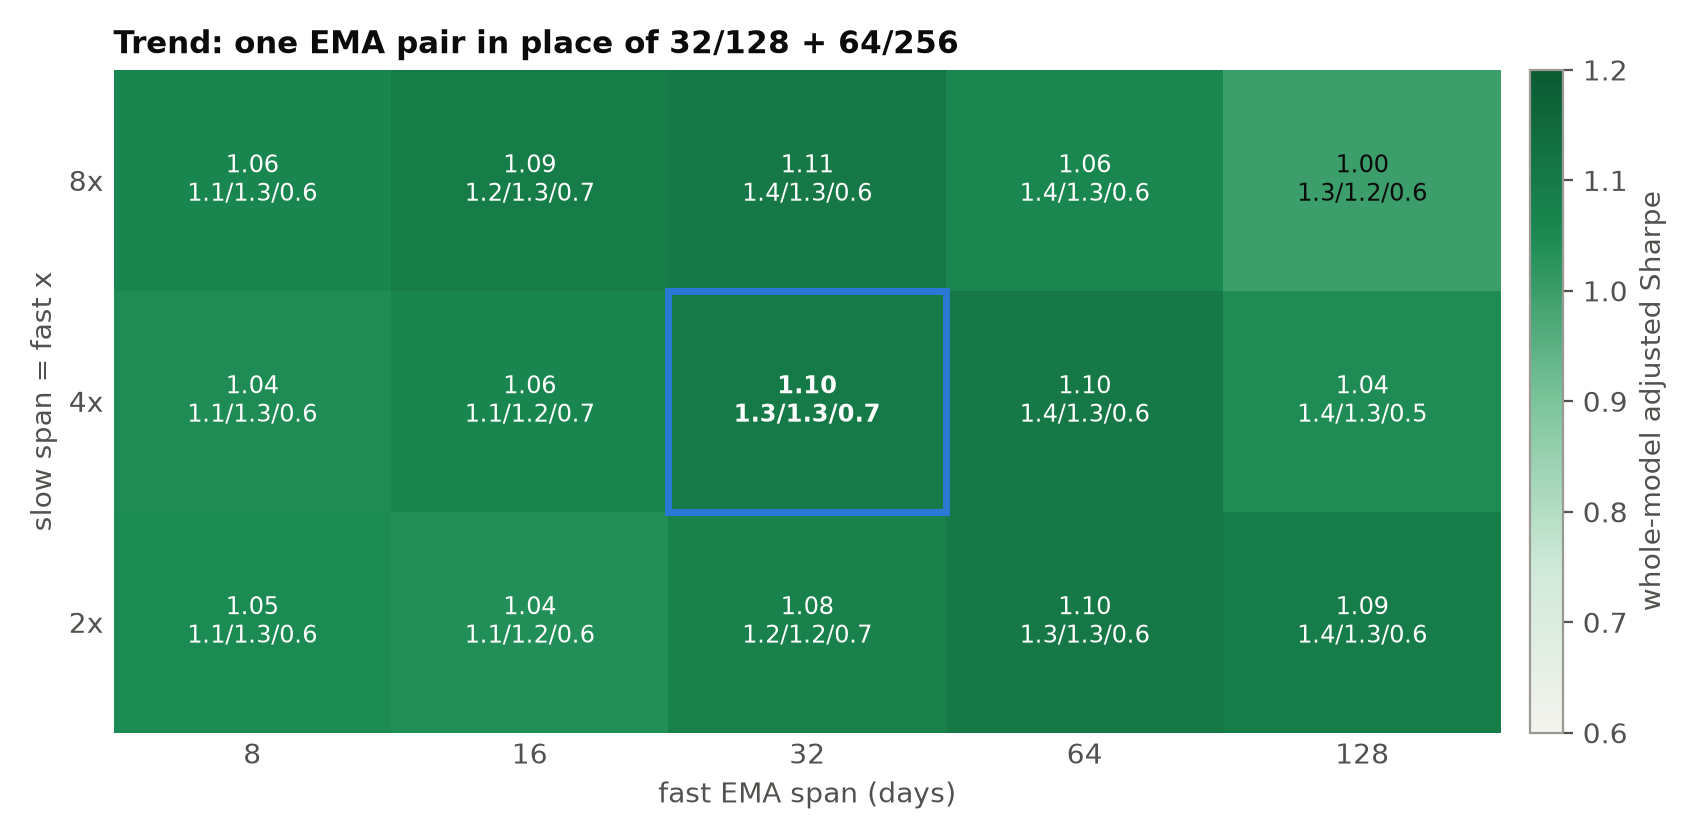
\includegraphics[width=0.86\linewidth]{fig_trend.png}\end{center}

\textbf{Inflation lookbacks.} Any stock lookback of 120 to 250 days scores 1.00 to 1.11, whatever the bond lookback. Only a 20-day stock lookback breaks it (0.63 to 0.75). That fits the mechanism: stocks react to persistent inflation, not to one month of noise.
\begin{center}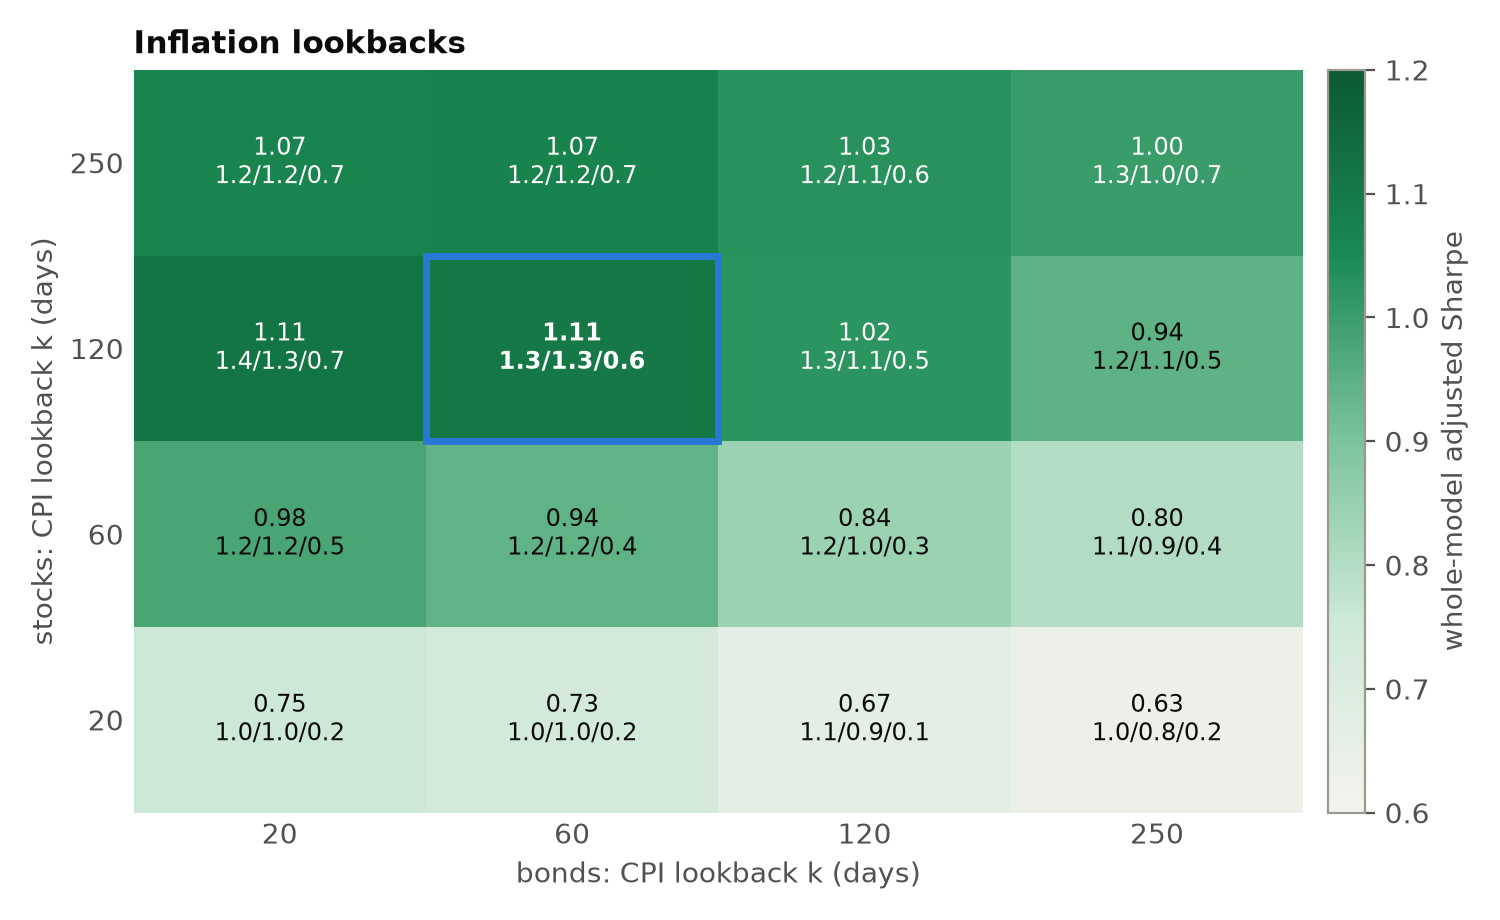
\includegraphics[width=0.7\linewidth]{fig_inflation.png}\end{center}

\textbf{Twins.} Any threshold from 0.7 to 0.9 with any spread window scores 1.00 to 1.15. At 0.6, pairs that are not real twins enter and the score drops to 0.81 to 0.87, which is the twins placebo again. The best cell (1.15) is not the one we use; we kept the round one-year window.
\begin{center}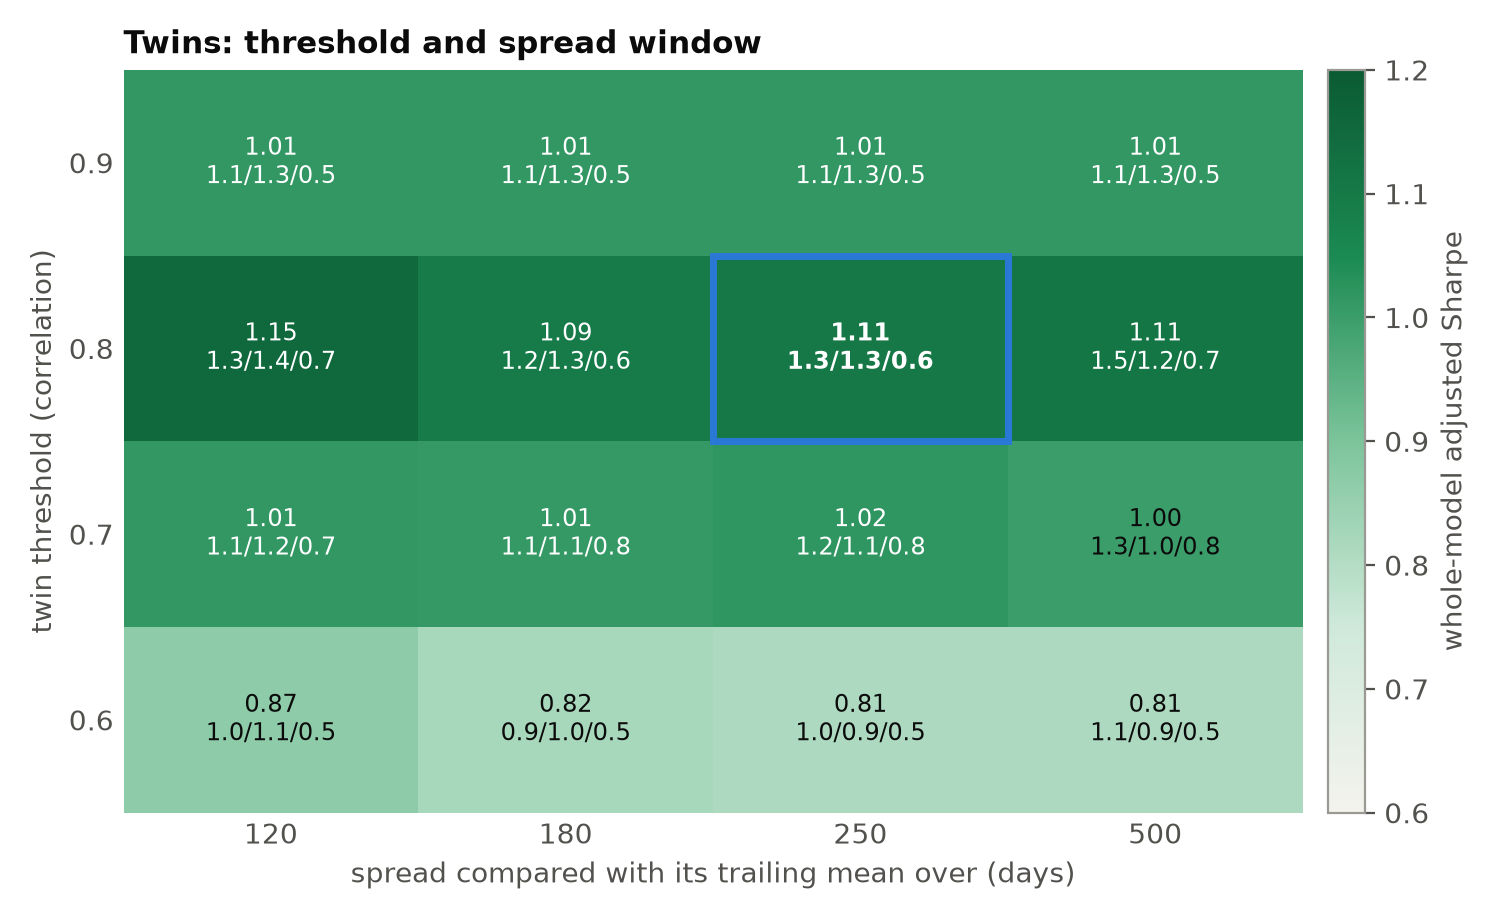
\includegraphics[width=0.7\linewidth]{fig_twins.png}\end{center}

\textbf{One setting at a time.} The green band is $\pm0.1$ around our score. Momentum lookback 1.03 to 1.11, inflation `normal' window 1.05 to 1.11, glide 1.02 to 1.11, sleeve risk window 1.08 to 1.11. Costs: 1.04 at twice Lynx's cost, 0.97 at three times.
\begin{center}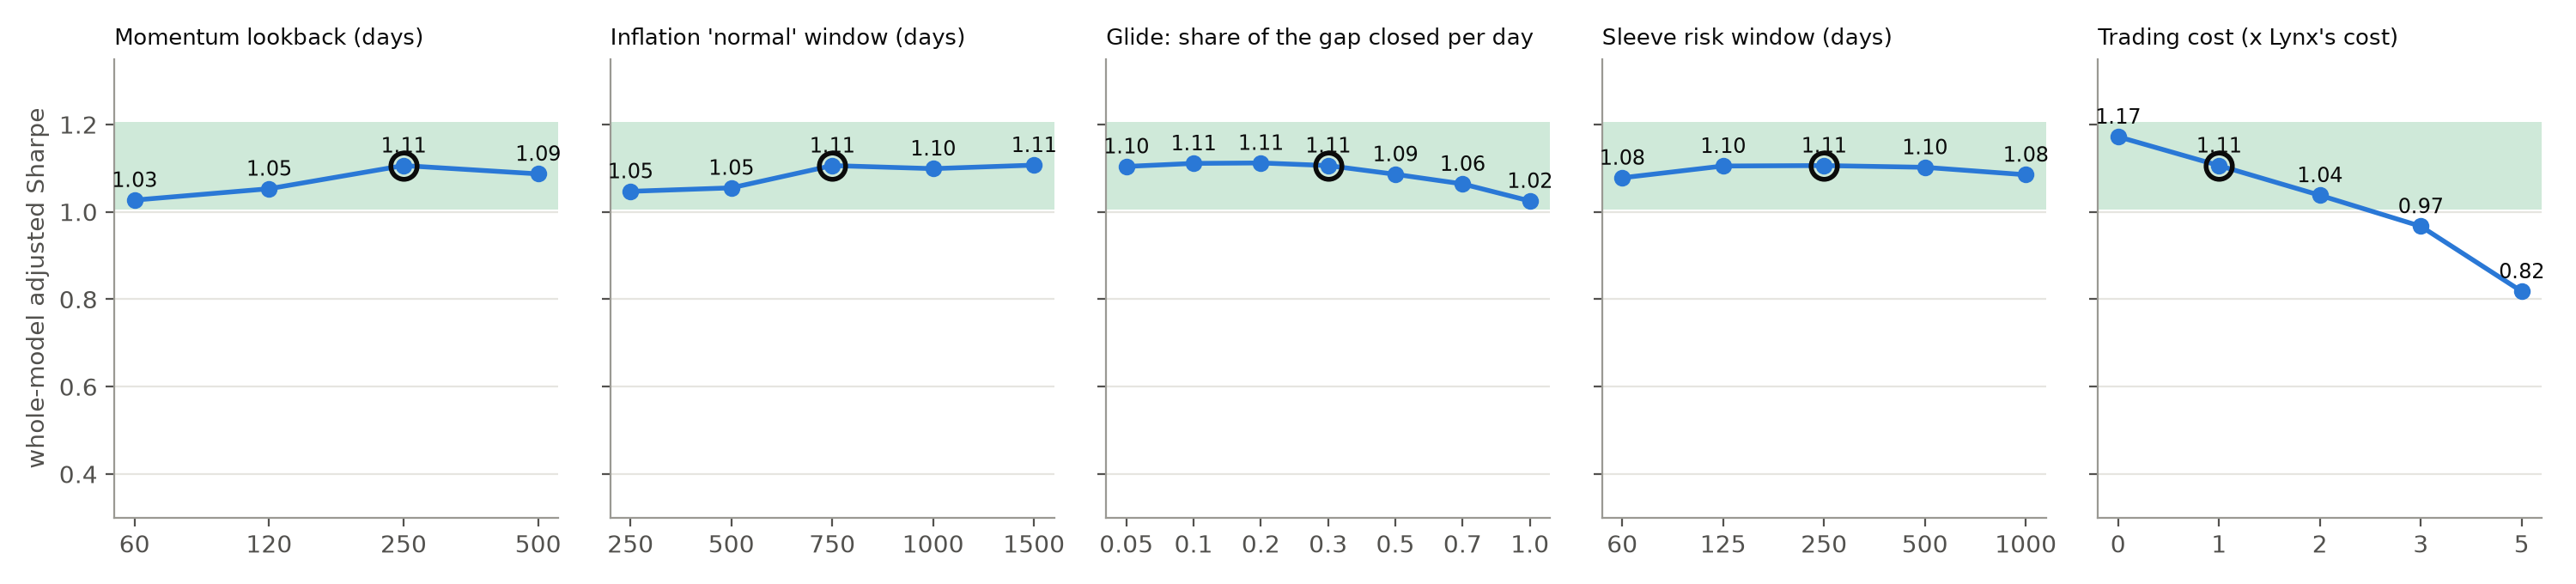
\includegraphics[width=\linewidth]{fig_1d.png}\end{center}

\section{Weak spots}
\begin{enumerate}
\item \textbf{2009--2016 is the softest era (0.63).} Trend stopped working there (the 2009 V-shaped reversal and the 2011--12 risk-on/risk-off swings), a known difficult period for trend followers. Inflation and twins held up.
\item \textbf{Twins lean on one pair.} Without beryllium the model scores 0.87.
\item \textbf{More cost-sensitive than a buy-and-hold book.} It holds positions 39 days on average; at twice Lynx's cost it still scores 1.04.
\item \textbf{We have seen all three eras.} Parameters are round numbers set up front, the one data-based choice (keeping twins) was made on 1997--2009, and the sweeps show a plateau. Only the out-of-sample period is a clean test.
\end{enumerate}

\section{Reproduce}
\begin{verbatim}
python BOMBASTRAT/bombastrat.py --prices data/close_prices_insample.csv \
       --macro data/macro_data_insample.csv --out positions.csv
python whitepaper/sweeps.py && python whitepaper/figures.py   # every number in Section 5
\end{verbatim}
The model is one file of about 100 lines (\texttt{BOMBASTRAT/bombastrat.py}); every parameter is a named constant at the top.

\end{document}
